
\section{Parametric Equations \& Polar Coordinates}
\begin{frame}{Parametric Equations}
    \begin{block}{Definition}
        Suppose that x and y are both given as functions of a third variable t
        (called a parameter) by the equations\\
        \begin{center}
            $x=f(t)$  $y=g(t)$
        \end{center}
    \end{block}
    \begin{center}
        $x=cost$ $y=sin t$ $(0 \leqslant t \leqslant 2\pi)$\\
    \end{center}
    If we plot points, it appears that the curve is a circle. We can confirm this
    impression by eliminating t. Observe that
    $$x^2+y^2=sin^2t +cos^2 t= 1$$
    Thus the point $(x,y)$ moves on the unit circle $x^2+y^2=1$. Notice that in
    this example the parameter t can be interpreted as the angle (in radians).
    As t increases from 0 to 2$\pi$, the point $(x,y) = (cost,sint)$ moves once
    around the circle in the counterclockwise direction starting from the point
    $(1,0)$.
\end{frame}

\begin{frame}{A Typical Example: Cycloid}
    \begin{block}{Definition}
        The curve traced out by a point on the circumference of a circle as the
        circle rolls along a straight line is called a cycloid .
        Therefore parametric equations of the cycloid are
        \begin{center}
            $x=r(\theta-sin\theta)$ $y=r(1-cos\theta)$ $ \theta \in R$
        \end{center}
    \end{block}
    \begin{center}
        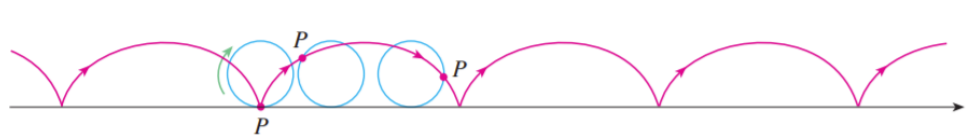
\includegraphics[width=0.95\linewidth]{res/Cycloid.png}
    \end{center}
\end{frame}

\begin{frame}{Polar Coordinates}
    We choose a point in the plane that is called the pole (or origin) and is
    labeled O. Then we draw a ray (half-line) starting at O called the polar
    axis. This axis is usually drawn horizontally to the right and corresponds
    to the positive x-axis in Cartesian coordinates.\\
    If P is any other point in the plane, let r be the distance from O to P and
    let $\theta$ be the angle (usually measured in radians) between the polar axis and the line OP as in Figure 1 . Then the point P is represented by the
    ordered pair $(r,\theta)$ and r,$\theta$ are called polar coordinates of P. We use the convention that an angle is positive if measured in the counterclockwise direction from the polar axis and negative in the clockwise direction. If P = O, then $r = 0$ and we agree that $(0,\theta)$ represents the pole for any value of $\theta$.
\end{frame}
\begin{frame}{Polar Coordinates}
    \begin{figure}[htb]
        \centering
        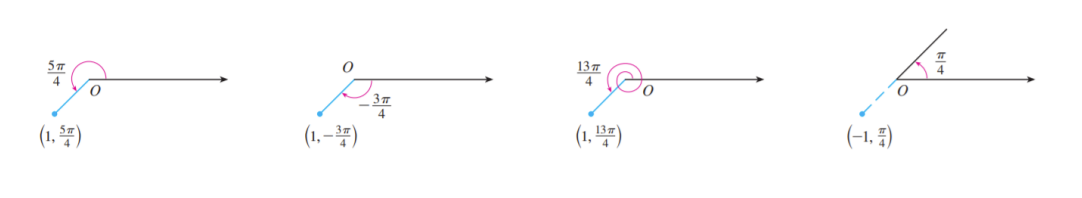
\includegraphics[width=0.95\linewidth]{res/polar.png}
    \end{figure}
    In fact, since a complete counterclockwise rotation is given by an angle
    $2\pi$, the point represented by polar coordinates $(r,\theta)$ is also represented by\\
    \begin{center}
        $(r,\theta+2n\pi)$ and $(-r,\theta+(2n+1)\pi)$
    \end{center}
\end{frame}

\colortheme{blue!50!black}
\begin{frame}{Polar Coordinates and Cartesian Coordinates}
    \begin{block}{Relationship between Polar Coordinates and Cartesian Coordinates}
        \begin{center}
            $x=r cos\theta$  $y=r sin \theta$\\
            $r^2=x^2+y^2$  $tan\theta = \frac{y}{x}$
        \end{center}
    \end{block}
\end{frame}

\colortheme{pink!100!black}
\begin{frame}{Cartesian coordinates and Cylindrical coordinates}
    \begin{block}{cylindrical to Cartesian coordinates}
        \begin{center}
            $x=r cos \phi$\\
            $y=r sin \phi$\\
            $z=z$
        \end{center}
    \end{block}
    \begin{block}{inverse relations (from Cartesian to cylindrical coordinates) }
        \begin{center}
            $r=\sqrt{x^2+y^2}$\\
            $tan \phi=\frac{y}{x}$\\
            $z=z$
        \end{center}
    \end{block}
\end{frame}

\begin{frame}{Cartesian coordinates and Spherical coordinates}
    \begin{block}{spherical to Cartesian coordinates}
        \begin{center}
            $x=r sin \theta cos \phi$\\
            $y=r sin\theta sin \phi$\\
            $z=r cos\theta$
        \end{center}
    \end{block}
    \begin{block}{inverse relations (from Cartesian to spherical coordinates) }
        \begin{center}
            $r=\sqrt{x^2+y^2+z^2}$\\
            $tan \phi=\frac{y}{x}$\\
            $tan \theta=\frac{\sqrt{x^2+y^2}}{z}$
        \end{center}
    \end{block}
\end{frame}

\begin{frame}{Cardioid}
    \begin{block}{Definition}
        - parametric representation:
        \begin{center}
            $x(\theta)=2a(1-cos \theta)cos \theta$\\
            $y(\theta)=2a(1-cos \theta)sin \theta$\\
            $(0\leqslant \theta \leqslant 2\pi)$
        \end{center}
        - polar coordinates:
        \begin{center}
            $r =2a(1-cos \theta)$\\
            $(0\leqslant \theta \leqslant 2\pi)$
        \end{center}
        Cardioid is special Cycloid and special Limaçon
    \end{block}
\end{frame}

\begin{frame}{Cardioid}
    \begin{block}{Cardioid}
        \begin{center}
            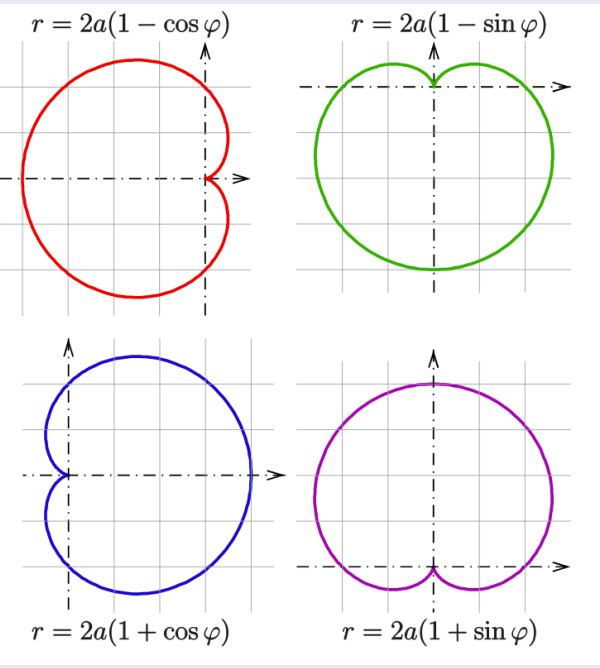
\includegraphics[width=0.5\linewidth]{res/Cardioid.png}
        \end{center}
    \end{block}
\end{frame}

\begin{frame}{Limaçon}
    \begin{block}{Definition}
        \begin{center}
            $r=1+c sin\theta$\\~\\
            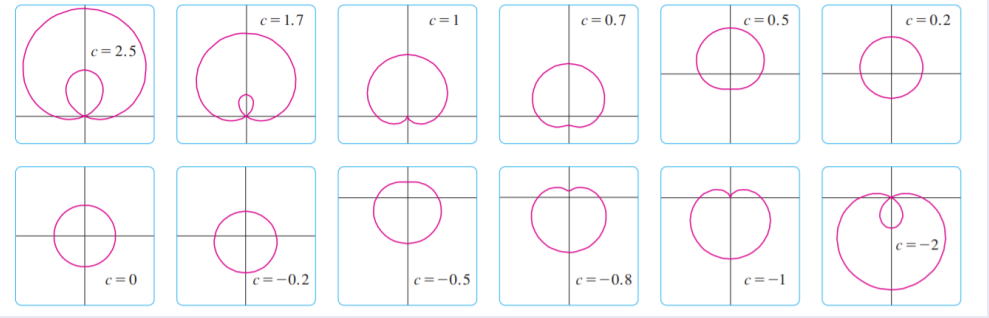
\includegraphics[width=0.85\linewidth]{res/limacon.png}
        \end{center}
    \end{block}
\end{frame}
\begin{frame}{Conchoid}
    \begin{block}{Definition}
        \begin{center}
            $r=1+c sec\theta$\\~\\
            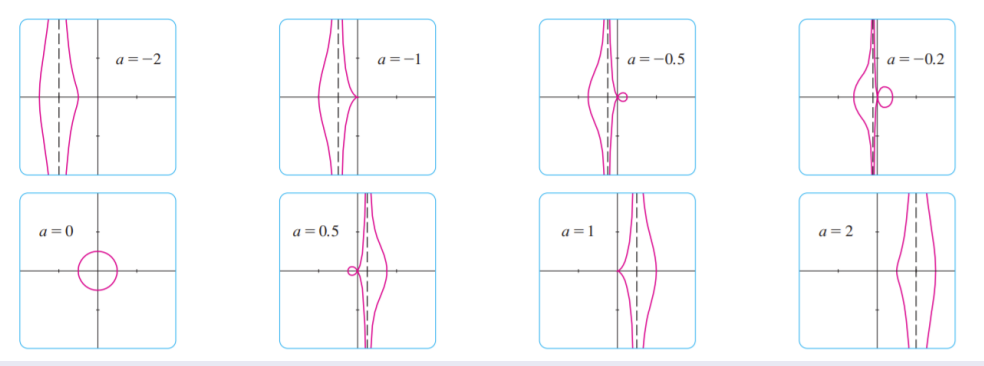
\includegraphics[width=0.85\linewidth]{res/Conchoid.png}
        \end{center}
    \end{block}
\end{frame}
\begin{frame}{Epicycloid}
    \begin{block}{Definition}
        \begin{center}
            $x(\theta)=(R+r)cos\theta-r cos(\frac{R+r}{r}\theta)$\\
            $y(\theta)=(R+r)sin\theta-r sin(\frac{R+r}{r}\theta)$\\~\\
            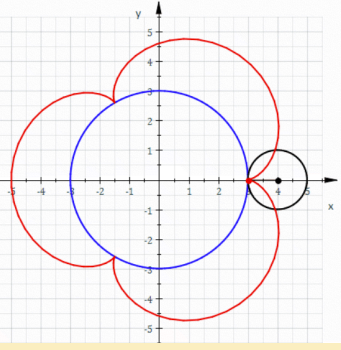
\includegraphics[width=0.55\linewidth]{res/Epicycloid.png}
        \end{center}
    \end{block}
\end{frame}
\begin{frame}{Epitrochoid}
    \begin{block}{Definition}
        \begin{center}
            $x(\theta)=(R+r)cos\theta-d cos(\frac{R+r}{r}\theta)$\\
            $y(\theta)=(R+r)sin\theta-d sin(\frac{R+r}{r}\theta)$\\~\\
            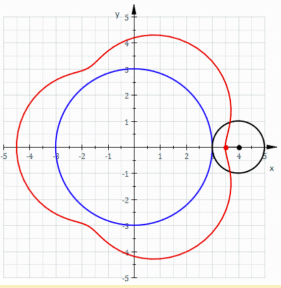
\includegraphics[width=0.55\linewidth]{res/Epitrochoid.png}
        \end{center}
    \end{block}
\end{frame}
\begin{frame}{Hypocycloid}
    \begin{block}{Definition}
        \begin{center}
            $x(\theta)=(R-r)cos\theta-r cos(\frac{R-r}{r}\theta)$\\
            $y(\theta)=(R-r)sin\theta-r sin(\frac{R-r}{r}\theta)$\\~\\
            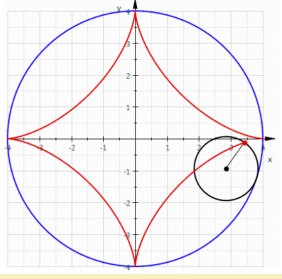
\includegraphics[width=0.55\linewidth]{res/Hypocycloid.png}
        \end{center}
    \end{block}
\end{frame}
\begin{frame}{Hypotrochoid}
    \begin{block}{Definition}
        \begin{center}
            $x(\theta)=(R-r)cos\theta-d cos(\frac{R-r}{r}\theta)$\\
            $y(\theta)=(R-r)sin\theta-d sin(\frac{R-r}{r}\theta)$\\~\\
            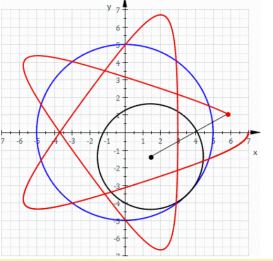
\includegraphics[width=0.55\linewidth]{res/Hypotrochoid.png}
        \end{center}
    \end{block}
\end{frame}

\begin{frame}{Bézier curves}
    \begin{block}{Definition}
        Bézier curves are used in computer-aided design and are named after the
        French mathematician Pierre Bézier (1910-1999), who worked in the
        automotive industry. A cubic Bézier curve is determined by four control
        points, $P_0 (x_0,y_0)$,$P_1 (x_1,y_1)$,$P_2 (x_2,y_2)$, and $P_3 (x_3,y_3)$, and is defined by the parametric equations:
        \begin{center}
            $x=x_0 (1-t)^3 + 3x_1 t(1-t)^2 + 3x_2 t^2(1-t)+ x_3 t^3$\\
            $y=y_0 (1-t)^3 + 3y_1 t(1-t)^2 + 3x_2 t^2(1-t)+ y_3 t^3$
        \end{center}
    \end{block}
    More Details: https://zhuanlan.zhihu.com/p/471457420
\end{frame}

\begin{frame}{Application of Bézier Curves in desmos}
    \begin{center}
        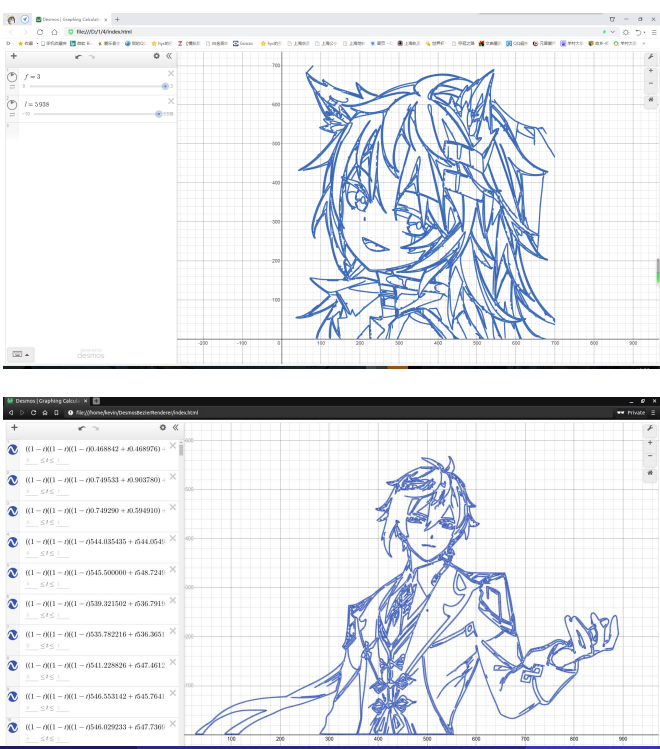
\includegraphics[width=0.6\linewidth]{res/demo1.png}
    \end{center}
\end{frame}
\begin{frame}{Application of Bézier Curves in desmos}
    \begin{center}
        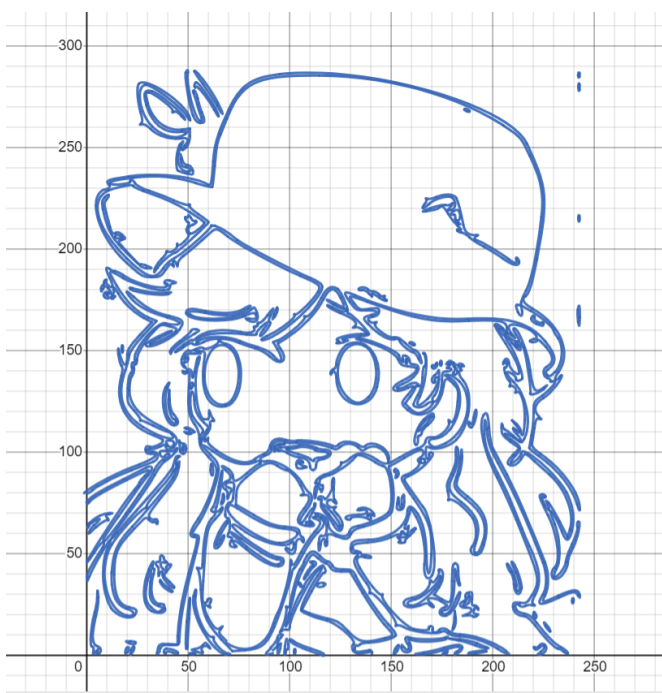
\includegraphics[width=0.6\linewidth]{res/demo2.png}
    \end{center}
\end{frame}
\begin{frame}{Application of Bézier Curves in desmos}
    \begin{center}
        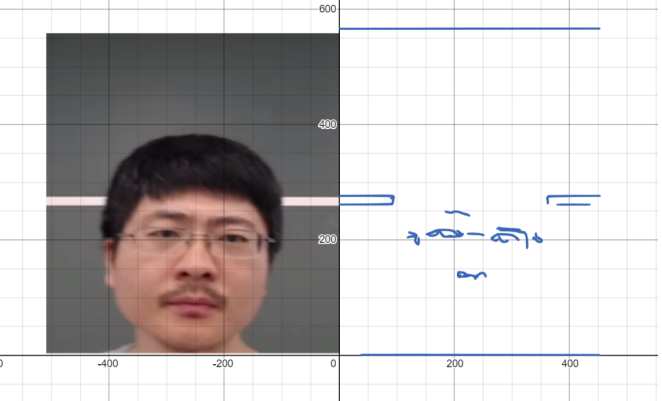
\includegraphics[width=0.75\linewidth]{res/demo.png}
    \end{center}
\end{frame}

\colortheme{green!30!black}
\begin{frame}{Tangents}
    \begin{block}{Slope of the Tangent Line with Parametric Curves}
        $$\frac{dy}{dx}=\frac{\frac{dy}{dt}}{\frac{dx}{dt}}$$
    \end{block}
    For the second order derivative, we have:\\
    $$\frac{d^2y}{dx^2}=\frac{d}{dx}\frac{dy}{dx}=\frac{\frac{d}{dt}\frac{dy}{dx}}{\frac{dx}{dt}}$$
\end{frame}

\begin{frame}{Area and Arc Length}
    \begin{block}{Area}
        We know that the area under a curve $y = F(x)$ from $a$ to $b$ is
        $A = \int_a ^b F(x) dx$, where $F(x) \geqslant 0$. If the curve is traced out once by the parametric equations $x = f(t)$ and $y = g(t)$, $\alpha \leqslant t \leqslant \beta$, then we can calculate an area formula by using the Substitution Rule for Definite Integrals as follows:
        $$A=\int _a^b y dx = \int_{\alpha}^{\beta} g(t) f^{\prime}(t) dt$$ or $$=\int^{\alpha}_{\beta} g(t) f^{\prime}(t) dt$$
    \end{block}
\end{frame}

\begin{frame}{Arc Length}
    \begin{block}{Arc Length}
        If a curve C is described by the parametric equations $x = f(t)$,$y = g(t)$,$\alpha \leqslant t \leqslant \beta $, where $f^{\prime}$ and $g^{\prime}$ are continuous on $[\alpha,\beta]$ and C is traversed exactly once as t increases from$\alpha$ to $\beta$, then the length of C is
        $$L=\int_{\alpha}^{\beta}\sqrt{(\frac{dx}{dt})^2+(\frac{dy}{dt})^2} dt $$
    \end{block}
\end{frame}

\begin{frame}{Surface Area}
    \begin{block}{Surface Area}
        In the same way as for arc length, we can adapt to obtain a formula for
        surface area. If the curve given by the parametric equations $x = f(t)$,$y = g(t)$,$\alpha \leqslant t \leqslant \beta $ is rotated about the x-axis, where $f^{\prime}$ and $g^{\prime}$ are continuous and $g(t) \geqslant 0$, then the area of the resulting surface is given by
        $$ S=\int_{\alpha}^{\beta} 2\pi y\sqrt{(\frac{dx}{dt})^2+(\frac{dy}{dt})^2} dt $$
    \end{block}

\end{frame}

\colortheme{blue!50!black}
\begin{frame}{Tangents}
    \begin{block}{Slope of the Tangent Line with  Polar Coordinates}
        $$x=r cos\theta,y=r sin\theta$$
        where r can be regarded as a function of $\theta$. Hence we have
        $$\frac{dy}{dx}=\frac{\frac{dy}{d\theta}}{\frac{dx}{d\theta}}=\frac{\frac{dy}{d\theta}sin \theta + r cos\theta}{\frac{dy}{d\theta} cos\theta -r sin\theta}$$
    \end{block}
\end{frame}
\begin{frame}{Area And Arc Length}
    Suppose we have the function in polar coordinates:
    $$r=f(\theta),a \leqslant \theta \leqslant b$$
    For the area enclosed by this function, we have:
    $$A=\int_a^b \frac{1}{2}f^2(\theta)d\theta$$
    For the area enclosed by this function, we have:
    $$L=\int_a^b \sqrt{r^2+(\frac{dr}{d\theta})^2} d\theta$$
\end{frame}

\begin{frame}{Exercise 1}
    \begin{block}{tangents}
        Find equations of the tangents to the curve $x = 3t^2 +1, y = 2t^3 +1$ that
        pass through the point $(4,3)$.
    \end{block}
\end{frame}

\begin{frame}{Exercise 2}
    \begin{enumerate}
        \item Find the exact length of the curve
              \begin{center}
                  $x=1+3t^2$, $y=4+2t^3$, $0 \leqslant t \leqslant 1$
              \end{center}
        \item
              Find the area enclosed by the x-axis and the curve
              \begin{center}
                  $x=1+e^t$, $y=t-t^2$
              \end{center}
        \item
              Find the exact area of the surface obtained by rotating the given curve about the x-axis.
              \begin{center}
                  $x=3t-t^3$, $y=3t^2$, $0 \leqslant t \leqslant 1$
              \end{center}
    \end{enumerate}
\end{frame}

\begin{frame}{Exercise 3 }
    \begin{enumerate}
        \item Find the slope of the tangent line to the given polar curve at the point specified by the value of $\theta$
              \begin{center}
                  $r=2-sin\theta$, $\theta=\frac{\pi}{3}$
              \end{center}
        \item
              Find the area of the region enclosed by one loop of the curve:
              \begin{center}
                  $r=2 sin5\theta$
              \end{center}
    \end{enumerate}
\end{frame}

\begin{frame}{Answers}
    exercises 1:\\
    $\frac{dy}{dx}=\frac{\frac{dy}{dt}}{\frac{dx}{dt}}=\frac{6t^2}{6t}=t$\\
    when pass through $(4,3)$, we have $3-(2t^3+1)=t(4-(3t^2+1)) \Rightarrow t=1$ or $t=-2$\\
    $\Rightarrow y=x-1$ or $y=-2x+11$\\
\end{frame}
\begin{frame}{Answers}
    exercises 2:
    \begin{enumerate}
        \item
              $L=\int_0^1\sqrt{(\frac{dy}{dt})^2+(\frac{dx}{dt})^2} dt=\int_0^1 6t \sqrt{1+t^2}dt = \int_1^2 \sqrt{u}(\frac{1}{2}d u)= 3 \cdot \frac{3}{2} [u ^ {\frac{3}{2}}]|_1^2= 2(2\sqrt{2}-1)$
        \item
              The curve $x = 1+e^t$,$y = t-t^2=t(1-t)$ intersects the x-axis when $y = 0$, that is, when $t = 0$ and $t = 1$. The corresponding values of x are $2$ and $1+e$. The shaded area is given by
              $\int_2^{1+e} (y_T-y_B) dx = \int_0^1 (y(t)-0) x^{\prime}(t) dt=\int _0^1 (t-t^2)e^t dt $\\
              $=\int _0^1 t e^t dt - \int_0^1 t^2 \cdot e^t dt$
              $= 3\int_0^1 t e^t dt - t^2 e^t|_0^1$\\
              $=3((t-1)e^t)|_0^1 - e =3-e$
        \item
              $x=3t-t^3$,$y=3t^2$,$0 \leqslant t \leqslant 1$.\\
              $(\frac{dx}{dt})^2+(\frac{dy}{dt})^2=(3-3t^2)^2+(6t)^2=(3(1+t)^2)^2$\\
              $S=\int_0^1 2\pi \cdot 3t^2 \cdot (1+t^2) dt$\\
              $=18\pi(\frac{1}{3} t^3 + \frac{1}{5} t^5)|_0^1$\\
              $=\frac{48}{5}\pi$
    \end{enumerate}
\end{frame}

\begin{frame}{Answers}
    \begin{enumerate}
        \item
              $x=r cos\theta= (2-sin\theta)cos\theta$,$y=r sin\theta =(2-sin\theta) sin\theta$\\
              $\frac{dy}{dx}=\frac{2cos\theta-sin2\theta}{-2sin\theta-cos2\theta}$\\
              when $\theta = \frac{\pi}{3}$, $\frac{dy}{dx}=\frac{2-\sqrt{3}}{1-2\sqrt{3}}$
        \item
              $sin 5\theta= 0 \Rightarrow 5\theta=n\pi \Rightarrow \theta=\frac{\pi}{5} n$\\
              $A=\int_0^{\frac{\pi}{5}} \frac{1}{2}(2sin5\theta)^2 d\theta$\\
              $=2 \int_0^{\frac{\pi}{5}}\frac{1}{2}(1-cos10\theta)|_0^{\frac{\pi}{5}}=\frac{\pi}{5}$\\
    \end{enumerate}
\end{frame}

\begin{frame}{Reference}
    1. Huang, Jiahe. VV156 RC4.pdf.2022.\\
    2. Huang, Yucheng. VV156 RC6.pdf. 2021.\\
    3. Chen, Jixiu et al. Mathematical Analysis (3rd Version). 2019\\
    4. Li, Junhao. VV156 RC5.pdf.2022.
\end{frame}

